\documentclass[a4paper,12pt]{article}
\usepackage[fleqn]{amsmath}
\usepackage{amssymb}
\usepackage{graphicx}
\graphicspath{ {./images/} }
\newcommand\longdiv[2]{%
$\strut#1$\kern.25em\smash{\raise.3ex\hbox{$\big)$}}$\mkern-8mu
        \overline{\enspace\strut#2}$}
\begin{document}

\title{Polynomials}	
\author{Edward Jex}
\maketitle
The order / degree of a polynomial is the highest power of the variable it contains. For example, a polynomial is order 3. \\
\section*{Division}
Long division is the best method when it is not known if there is a remainder or not. Otherwise it can  be done by inspection. \\
\subsection*{Example 1}
Divide $2x^3 -3x^2 + x -6$ by $x-2$ \\\\
\phantom{A}\hspace{0.8cm} $2x^2 + x + 3$ \\
\longdiv{x-2}{2x^3 -3x^2 + x -6} \\
\phantom{A}\hspace{0.3cm} $-(2x^3 -4x^2)$ \\
\phantom{A}\hspace{2.1cm} $x^2$ \\
\phantom{A}\hspace{1.6cm} $-(x^2-2x)$ \\
\phantom{A}\hspace{3cm} $3x-6$ \\
\phantom{A}\hspace{2.5cm} $-(3x-6)$ \\
\phantom{A}\hspace{4cm} $0$ \\\\
$\Rightarrow 2x^3 -3x^2 + x -6 = (2x^2 + x + 3)(x-2)$
\section*{The Factor Theorem}
We can use the factor theorem to help us to solve algebraic equations of order greater than 2. \\
The factor theorem is as follows: \\
If $(x-\alpha)$ is a factor of $f(x)$ then $f(\alpha) = 0$ and $\alpha$ is the root of the equation of $f(x) = 0$. \\
\subsection*{Example 2}
Show that $(x-1)$ is a linear factor of $2x^3 - 5x^2 - 6x + 9$ \\ 
\begin{align*}
f(1) = 0 & \Rightarrow (x-1) \text{is a factor by the factor theorum} \\
2x^3 - 5x^2 - 6x + 9 & = (x-1)(2x^2-3x-9) \\
& = (x-1)(2x+3)(x-3) \\
& \Rightarrow x = 1, -\frac{3}{2}, 3 \\
\end{align*}
\section*{Sketching Polynomials}
To sketch polynomials, we must find where it crosses the x-axis and y-axis. We also need to know what order the polynomial is so that we know the general shape.  \\
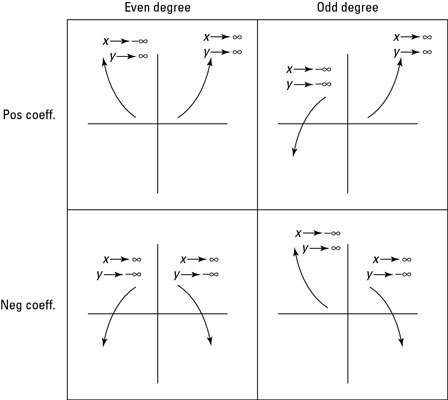
\includegraphics[scale=0.7]{Graphs}
\section*{Turning Points}
A point where the gradient is 0. If a polynomial is of order n, it can at most n-1 turning points. 
\end{document}